\documentclass[spanish,]{article}

\usepackage{lmodern}
\renewcommand*\familydefault{\sfdefault} %% Only if the base font of the document is to be sans serif
\usepackage[T1]{fontenc}

% \usepackage{hyperref}
% \hypersetup{colorlinks=true}

\usepackage{amssymb,amsmath}
\usepackage{ifxetex,ifluatex}
\usepackage{fixltx2e} % provides \textsubscript
\ifnum 0\ifxetex 1\fi\ifluatex 1\fi=0 % if pdftex
  \usepackage[T1]{fontenc}
  \usepackage[utf8]{inputenc}
\else % if luatex or xelatex
  \ifxetex
    \usepackage{mathspec}
  \else
    \usepackage{fontspec}
  \fi
  \defaultfontfeatures{Ligatures=TeX,Scale=MatchLowercase}
\fi
% use upquote if available, for straight quotes in verbatim environments
\IfFileExists{upquote.sty}{\usepackage{upquote}}{}
% use microtype if available
\IfFileExists{microtype.sty}{%
\usepackage{microtype}
\UseMicrotypeSet[protrusion]{basicmath} % disable protrusion for tt fonts
}{}
\usepackage{hyperref}
\PassOptionsToPackage{usenames,dvipsnames}{color} % color is loaded by hyperref
\hypersetup{unicode=true,
            pdftitle={Determinación de ambientes (PPR) y Cartas SGM en padrones rurales de Uruguay: Procesamiento de los mapas},
            pdfauthor={Juan Manuel Barreneche},
            colorlinks=true,
            linkcolor=Maroon,
            citecolor=Blue,
            urlcolor=Blue,
            breaklinks=true}
\urlstyle{same}  % don't use monospace font for urls
\ifnum 0\ifxetex 1\fi\ifluatex 1\fi=0 % if pdftex
  \usepackage[shorthands=off,main=spanish]{babel}
\else
  \usepackage{polyglossia}
  \setmainlanguage[]{spanish}
\fi
\usepackage{color}
\usepackage{fancyvrb}
\newcommand{\VerbBar}{|}
\newcommand{\VERB}{\Verb[commandchars=\\\{\}]}
\DefineVerbatimEnvironment{Highlighting}{Verbatim}{commandchars=\\\{\}}
% Add ',fontsize=\small' for more characters per line
\newenvironment{Shaded}{}{}
\newcommand{\KeywordTok}[1]{\textcolor[rgb]{0.00,0.44,0.13}{\textbf{{#1}}}}
\newcommand{\DataTypeTok}[1]{\textcolor[rgb]{0.56,0.13,0.00}{{#1}}}
\newcommand{\DecValTok}[1]{\textcolor[rgb]{0.25,0.63,0.44}{{#1}}}
\newcommand{\BaseNTok}[1]{\textcolor[rgb]{0.25,0.63,0.44}{{#1}}}
\newcommand{\FloatTok}[1]{\textcolor[rgb]{0.25,0.63,0.44}{{#1}}}
\newcommand{\ConstantTok}[1]{\textcolor[rgb]{0.53,0.00,0.00}{{#1}}}
\newcommand{\CharTok}[1]{\textcolor[rgb]{0.25,0.44,0.63}{{#1}}}
\newcommand{\SpecialCharTok}[1]{\textcolor[rgb]{0.25,0.44,0.63}{{#1}}}
\newcommand{\StringTok}[1]{\textcolor[rgb]{0.25,0.44,0.63}{{#1}}}
\newcommand{\VerbatimStringTok}[1]{\textcolor[rgb]{0.25,0.44,0.63}{{#1}}}
\newcommand{\SpecialStringTok}[1]{\textcolor[rgb]{0.73,0.40,0.53}{{#1}}}
\newcommand{\ImportTok}[1]{{#1}}
\newcommand{\CommentTok}[1]{\textcolor[rgb]{0.38,0.63,0.69}{\textit{{#1}}}}
\newcommand{\DocumentationTok}[1]{\textcolor[rgb]{0.73,0.13,0.13}{\textit{{#1}}}}
\newcommand{\AnnotationTok}[1]{\textcolor[rgb]{0.38,0.63,0.69}{\textbf{\textit{{#1}}}}}
\newcommand{\CommentVarTok}[1]{\textcolor[rgb]{0.38,0.63,0.69}{\textbf{\textit{{#1}}}}}
\newcommand{\OtherTok}[1]{\textcolor[rgb]{0.00,0.44,0.13}{{#1}}}
\newcommand{\FunctionTok}[1]{\textcolor[rgb]{0.02,0.16,0.49}{{#1}}}
\newcommand{\VariableTok}[1]{\textcolor[rgb]{0.10,0.09,0.49}{{#1}}}
\newcommand{\ControlFlowTok}[1]{\textcolor[rgb]{0.00,0.44,0.13}{\textbf{{#1}}}}
\newcommand{\OperatorTok}[1]{\textcolor[rgb]{0.40,0.40,0.40}{{#1}}}
\newcommand{\BuiltInTok}[1]{{#1}}
\newcommand{\ExtensionTok}[1]{{#1}}
\newcommand{\PreprocessorTok}[1]{\textcolor[rgb]{0.74,0.48,0.00}{{#1}}}
\newcommand{\AttributeTok}[1]{\textcolor[rgb]{0.49,0.56,0.16}{{#1}}}
\newcommand{\RegionMarkerTok}[1]{{#1}}
\newcommand{\InformationTok}[1]{\textcolor[rgb]{0.38,0.63,0.69}{\textbf{\textit{{#1}}}}}
\newcommand{\WarningTok}[1]{\textcolor[rgb]{0.38,0.63,0.69}{\textbf{\textit{{#1}}}}}
\newcommand{\AlertTok}[1]{\textcolor[rgb]{1.00,0.00,0.00}{\textbf{{#1}}}}
\newcommand{\ErrorTok}[1]{\textcolor[rgb]{1.00,0.00,0.00}{\textbf{{#1}}}}
\newcommand{\NormalTok}[1]{{#1}}
\usepackage{longtable,booktabs}
\usepackage{graphicx,grffile}
\makeatletter
\def\maxwidth{\ifdim\Gin@nat@width>\linewidth\linewidth\else\Gin@nat@width\fi}
\def\maxheight{\ifdim\Gin@nat@height>\textheight\textheight\else\Gin@nat@height\fi}
\makeatother
% Scale images if necessary, so that they will not overflow the page
% margins by default, and it is still possible to overwrite the defaults
% using explicit options in \includegraphics[width, height, ...]{}
\setkeys{Gin}{width=\maxwidth,height=\maxheight,keepaspectratio}
\IfFileExists{parskip.sty}{%
\usepackage{parskip}
}{% else
\setlength{\parindent}{0pt}
\setlength{\parskip}{6pt plus 2pt minus 1pt}
}
\setlength{\emergencystretch}{3em}  % prevent overfull lines
\providecommand{\tightlist}{%
  \setlength{\itemsep}{0pt}\setlength{\parskip}{0pt}}
\setcounter{secnumdepth}{0}
% Redefines (sub)paragraphs to behave more like sections
\ifx\paragraph\undefined\else
\let\oldparagraph\paragraph
\renewcommand{\paragraph}[1]{\oldparagraph{#1}\mbox{}}
\fi
\ifx\subparagraph\undefined\else
\let\oldsubparagraph\subparagraph
\renewcommand{\subparagraph}[1]{\oldsubparagraph{#1}\mbox{}}
\fi

\title{Determinación de ambientes (PPR) y Cartas SGM en padrones rurales de
Uruguay: Procesamiento de los mapas}
\author{Juan Manuel Barreneche}
\date{}

\begin{document}
\maketitle

\section{Resumen}\label{resumen}

En este texto se describe el proceso de creación de las tablas que
vinculan Padrones Rurales con Ambientes y con Cartas SGM. Decidí meter
el código todo junto en este archivo, en vez de tener varios scripts
separados, porque así se conforma un tutorial. En el futuro tal vez sea
mejor volver a muchos archivos individuales.

De todas formas tener todo en un único texto ayuda a visualizar el hilo
conductor.

Nótese que acá hay código de SQL, GRASS y Bash, como mínimo.

El esquema del producto final está en el archivo \texttt{BioUy.xml} y se
puede visualizar en \href{https://www.draw.io/}{https://www.draw.io}. En
la \textbf{Figura 1} se muestra el esquema resultante.

\begin{figure}[htbp]
\centering
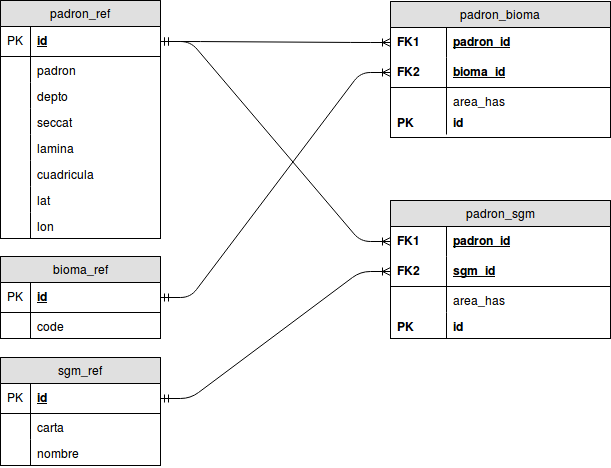
\includegraphics{https://raw.githubusercontent.com/jumanbar/BioUy/master/Clean/BioUy.png}
\caption{Modelo Entidad Relación}
\end{figure}

\newpage

\section{Arreglos de la capa vectorial en
PostgreSQL}\label{arreglos-de-la-capa-vectorial-en-postgresql}

Lo primero es hacer varios arreglos a la capa vectorial con los
ambientes (\texttt{ppr\_biomes}). Se asume que dicha capa ya está
importada dentro de la base.

Si hace falta importar la capa de nuevo, se puede hacer con QGIS: si se
lo conecta a la base PostgreSQL y con la interfaz gráfica se hace la
importación. Ver herramientas en el menú Database \textgreater{} DB
Manager.

A continuación se muestra la secuencia de pasos para modificar la capa
vectorial/tabla para disminuir la cantidad de errores topológicos y
complejidad. Esto ayuda a que se pueda renderizar más rápidamente en
QGIS y también a que hayan menos errores cuando se haga la exportación a
raster (GeoTIFF).

\subsection{1. Respaldo de la tabla
original}\label{respaldo-de-la-tabla-original}

Para hacer modificaciones primero se respalda la capa/tabla original,
bajo el nombre \texttt{ppr\_biomes\_bak} (este puede ser el nombre dado
a la capa al ser importada desde QGIS). Luego se crea una copia que
modificaremos, a la que llamamos \texttt{ppr\_biomes}:

\begin{Shaded}
\begin{Highlighting}[]
\KeywordTok{CREATE} \KeywordTok{TABLE} \NormalTok{ppr_biomes }\KeywordTok{AS} 
  \KeywordTok{SELECT} \KeywordTok{id}\NormalTok{, geom }\KeywordTok{FROM} \NormalTok{ppr_biomes_bak;}
\CommentTok{-- SELECT 48523}

\KeywordTok{ALTER} \KeywordTok{TABLE} \NormalTok{ppr_biomes }\KeywordTok{ADD} \KeywordTok{constraint} \NormalTok{pk_ppr_biomes_id }\KeywordTok{PRIMARY} \KeywordTok{KEY} \NormalTok{(}\KeywordTok{id}\NormalTok{);}

\KeywordTok{CREATE} \KeywordTok{INDEX} \NormalTok{sidx_ppr_biomes_geom }\KeywordTok{ON} \NormalTok{ppr_biomes }\KeywordTok{USING} \NormalTok{GIST (geom);}
\end{Highlighting}
\end{Shaded}

\subsection{2. Eliminar puntos
repetidos}\label{eliminar-puntos-repetidos}

\begin{Shaded}
\begin{Highlighting}[]
\KeywordTok{UPDATE} \NormalTok{ppr_biomes }\KeywordTok{SET} \NormalTok{geom = ST_RemoveRepeatedPoints(geom);}
\end{Highlighting}
\end{Shaded}

\begin{quote}
Query returned successfully: 48523 rows affected, 04:03 minutes
execution time.
\end{quote}

\subsection{3. Simplificar geometrías}\label{simplificar-geometruxedas}

En PostgreSQL:

\begin{Shaded}
\begin{Highlighting}[]
\KeywordTok{UPDATE} \NormalTok{ppr_biomes }\KeywordTok{SET} \NormalTok{geom = ST_Simplify(geom, }\DecValTok{1}\NormalTok{);}
\end{Highlighting}
\end{Shaded}

\subsection{4. Multi -\textgreater{} Single polygons
(ST\_Dump)}\label{multi---single-polygons-stux5fdump}

\begin{Shaded}
\begin{Highlighting}[]
\KeywordTok{CREATE} \KeywordTok{TABLE} \NormalTok{ppr_biomes_dump }\KeywordTok{AS}
  \KeywordTok{SELECT} \KeywordTok{id}\NormalTok{, (ST_Dump(geom)).* }\KeywordTok{from} \NormalTok{ppr_biomes;}
\CommentTok{-- SELECT 6798778}
\end{Highlighting}
\end{Shaded}

\subsection{5. Filtrar areas menores a una
hectárea}\label{filtrar-areas-menores-a-una-hectuxe1rea}

\subsubsection{5.1 Crear función filter\_rings en
PostgreSQL}\label{crear-funciuxf3n-filterux5frings-en-postgresql}

Sirve para eliminar áreas pequeñas.

Author: Simon Greener Web Page:
http://www.spatialdbadvisor.com/postgis\_tips\_tricks/92/filtering-rings-in-polygon-postgis/

\begin{quote}
Notes: This version of the function does not handle MultiPolygon
geometries. I choosed it because it performs better. I'm not sure if his
latest version (which does handle MultiPoligon) is really worse
performing even when dealing with single Polygons.
\end{quote}

Tiene una modificación del original: en vez de
\texttt{\textgreater{}\ \$2}, cambié por \texttt{\textgreater{}=\ \$2}.

\begin{Shaded}
\begin{Highlighting}[]
\KeywordTok{CREATE} \KeywordTok{OR} \KeywordTok{REPLACE} \KeywordTok{FUNCTION} \NormalTok{filter_rings(geometry, }\DataTypeTok{DOUBLE} \DataTypeTok{PRECISION}\NormalTok{)}
  \NormalTok{RETURNS geometry }\KeywordTok{AS}
\NormalTok{$BODY$}
\KeywordTok{SELECT} \NormalTok{ST_MakePolygon((}\CommentTok{/* Get outer ring of polygon */}
        \KeywordTok{SELECT} \NormalTok{ST_ExteriorRing(geom) }\KeywordTok{AS} \NormalTok{outer_ring}
          \KeywordTok{FROM} \NormalTok{ST_DumpRings($}\DecValTok{1}\NormalTok{)}
          \KeywordTok{WHERE} \NormalTok{path[}\DecValTok{1}\NormalTok{] = }\DecValTok{0} \CommentTok{/* ie the outer ring */}
        \NormalTok{),  }\DataTypeTok{ARRAY}\NormalTok{(}\CommentTok{/* Get all inner rings > a particular area */}
        \KeywordTok{SELECT} \NormalTok{ST_ExteriorRing(geom) }\KeywordTok{AS} \NormalTok{inner_rings}
          \KeywordTok{FROM} \NormalTok{ST_DumpRings($}\DecValTok{1}\NormalTok{)}
          \KeywordTok{WHERE} \NormalTok{path[}\DecValTok{1}\NormalTok{] > }\DecValTok{0} \CommentTok{/* ie not the outer ring */}
            \KeywordTok{AND} \NormalTok{ST_Area(geom) >= $}\DecValTok{2}
        \NormalTok{) ) }\KeywordTok{AS} \NormalTok{final_geom}
\NormalTok{$BODY$}
  \NormalTok{LANGUAGE }\StringTok{'sql'} \NormalTok{IMMUTABLE;}
\end{Highlighting}
\end{Shaded}

\subsubsection{5.2 Usar la función para eliminar áreas
pequeñas}\label{usar-la-funciuxf3n-para-eliminar-uxe1reas-pequeuxf1as}

\begin{Shaded}
\begin{Highlighting}[]
\CommentTok{-- drop table ppr_biomes_dump_filtered ;}
\KeywordTok{CREATE} \KeywordTok{TABLe} \NormalTok{ppr_biomes_dump_filtered }\KeywordTok{AS}
\KeywordTok{SELECT} \KeywordTok{id}\NormalTok{, path[}\DecValTok{1}\NormalTok{], filter_rings(geom, }\FloatTok{1e4}\NormalTok{) }\KeywordTok{AS} \NormalTok{geom }
  \KeywordTok{FROM} \NormalTok{ppr_biomes_dump}
 \KeywordTok{WHERE} \NormalTok{st_area(geom) > }\FloatTok{1e4}\NormalTok{;}
\CommentTok{-- SELECT 431296}
\end{Highlighting}
\end{Shaded}

Para hechar un vistazo:

\begin{Shaded}
\begin{Highlighting}[]
\KeywordTok{SELECT} \KeywordTok{id}\NormalTok{, path, st_npoints(geom), st_area(geom) }
  \KeywordTok{FROM} \NormalTok{ppr_biomes_dump_filtered}
 \KeywordTok{ORDER} \KeywordTok{BY} \NormalTok{st_area(geom) }\CommentTok{-- Para ver el área mínima de los poly}
 \KeywordTok{LIMIT} \DecValTok{10}\NormalTok{;}
\end{Highlighting}
\end{Shaded}

Crear índice en la tabla, creando la columna gid

\begin{Shaded}
\begin{Highlighting}[]
\KeywordTok{ALTER} \KeywordTok{TABLE} \NormalTok{ppr_biomes_dump_filtered }\KeywordTok{ADD} \KeywordTok{COLUMN} \NormalTok{gid SERIAL }\KeywordTok{PRIMARY} \KeywordTok{KEY}\NormalTok{;}
\KeywordTok{CREATE} \KeywordTok{INDEX} \NormalTok{sidx_ppr_biomes_dump_filtered_geom }
    \KeywordTok{ON} \NormalTok{ppr_biomes_dump_filtered }\KeywordTok{USING} \NormalTok{GIST (geom);}
\end{Highlighting}
\end{Shaded}

\subsection{6. Buffer}\label{buffer}

Este es un truco para solucionar problemas de polígonos interceptándose
a sí mismos.

\begin{Shaded}
\begin{Highlighting}[]
\KeywordTok{EXPLAIN} \KeywordTok{ANALYZE} \KeywordTok{UPDATE} \NormalTok{ppr_biomes_dump_filtered }
  \KeywordTok{SET} \NormalTok{geom = ST_Buffer(geom, }\DecValTok{0}\NormalTok{) \textbackslash{}g salida.txt}
\CommentTok{-- 3'42"}
\end{Highlighting}
\end{Shaded}

El problema de este truco es que genera geometrías MultiPolygon (96 de
431296). Se puede verificar si hay o no con este comando:

\begin{Shaded}
\begin{Highlighting}[]
\KeywordTok{SELECT} \FunctionTok{COUNT}\NormalTok{(*), st_GeometryType(geom) }
  \KeywordTok{FROM} \NormalTok{ppr_biomes_dump_filtered }
 \KeywordTok{GROUP} \KeywordTok{BY} \NormalTok{st_GeometryType(geom);}
\end{Highlighting}
\end{Shaded}

Debido a esto es que se ejecutan los comandos de la siguiente
sección\ldots{}

\subsection{7. Multi -\textgreater{} Single Polygon parte
2}\label{multi---single-polygon-parte-2}

Este paso hace 2 cosas:

\begin{enumerate}
\def\labelenumi{\arabic{enumi}.}
\tightlist
\item
  Rompe los ST\_MultiPolygon en pedazos simples, dejando objetos de
  clase ST\_Polygon solamente.
\item
  Elimina polígonos de área menor a 1 hectárea.
\end{enumerate}

Tabla chica, con sólo los MultiPolygon, convertidos en ``single'':

\begin{Shaded}
\begin{Highlighting}[]
\KeywordTok{CREATE} \KeywordTok{TABLE} \NormalTok{ppr_biomes_dump2 }\KeywordTok{AS}
\KeywordTok{SELECT} \KeywordTok{id}\NormalTok{, path }\KeywordTok{AS} \NormalTok{path0, (ST_Dump(geom)).*, gid }\CommentTok{-- gid = nextval?}
  \KeywordTok{FROM} \NormalTok{ppr_biomes_dump_filtered}
 \KeywordTok{WHERE} \NormalTok{ST_GeometryType(geom) = }\StringTok{'ST_MultiPolygon'}\NormalTok{;}
\end{Highlighting}
\end{Shaded}

Usar los \texttt{gid} en la tabla chica, para sacar los Multi de la
tabla original:

\begin{Shaded}
\begin{Highlighting}[]
\KeywordTok{DELETE} \KeywordTok{FROM} \NormalTok{ppr_biomes_dump_filtered }
 \KeywordTok{WHERE} \NormalTok{gid }\KeywordTok{IN} \NormalTok{(}\KeywordTok{SELECT} \NormalTok{gid }\KeywordTok{FROM} \NormalTok{ppr_biomes_dump2)}
    \KeywordTok{OR} \NormalTok{ST_Area(geom) < }\FloatTok{1e4}\NormalTok{;}
\end{Highlighting}
\end{Shaded}

De la tabla chica, sacamos los chicos (menores a 1 hectárea):

\begin{Shaded}
\begin{Highlighting}[]
\KeywordTok{DELETE} \KeywordTok{FROM} \NormalTok{ppr_biomes_dump2}
 \KeywordTok{WHERE} \NormalTok{ST_Area(geom) < }\FloatTok{1e4}\NormalTok{;}
\end{Highlighting}
\end{Shaded}

Metemos los polígonos de la tabla chica en la original. En dos pasos, ya
que hay que poner primero el polígono principal
(\texttt{path{[}1{]}\ =\ 1}) y luego los secundarios
(\texttt{path{[}1{]}\ \textless{}\textgreater{}\ 1}):

\begin{Shaded}
\begin{Highlighting}[]
\KeywordTok{INSERT} \KeywordTok{INTO} \NormalTok{ppr_biomes_dump_filtered}
  \KeywordTok{SELECT} \KeywordTok{id}\NormalTok{, path0 }\KeywordTok{AS} \NormalTok{path, geom, gid}
    \KeywordTok{FROM} \NormalTok{ppr_biomes_dump2}
   \KeywordTok{WHERE} \NormalTok{path[}\DecValTok{1}\NormalTok{] = }\DecValTok{1}\NormalTok{;}

\KeywordTok{INSERT} \KeywordTok{INTO} \NormalTok{ppr_biomes_dump_filtered}
\KeywordTok{SELECT} \KeywordTok{id}\NormalTok{, path0 }\KeywordTok{as} \NormalTok{path, geom, }
       \NormalTok{nextval(}\StringTok{'ppr_biomes_dump_filtered_gid_seq'}\NormalTok{) }\KeywordTok{AS} \NormalTok{gid}
  \KeywordTok{FROM} \NormalTok{ppr_biomes_dump2}
 \KeywordTok{WHERE} \NormalTok{path[}\DecValTok{1}\NormalTok{] <> }\DecValTok{1}\NormalTok{;}
\end{Highlighting}
\end{Shaded}

Checkeos de que esté todo bien\ldots{}

\begin{enumerate}
\def\labelenumi{\arabic{enumi}.}
\tightlist
\item
  No hay más MultiPolygons:
\end{enumerate}

\begin{Shaded}
\begin{Highlighting}[]
\KeywordTok{SELECT} \FunctionTok{count}\NormalTok{(*), st_GeometryType(geom) }
  \KeywordTok{FROM} \NormalTok{ppr_biomes_dump_filtered }
 \KeywordTok{GROUP} \KeywordTok{BY} \NormalTok{st_GeometryType(geom);}
\end{Highlighting}
\end{Shaded}

\begin{enumerate}
\def\labelenumi{\arabic{enumi}.}
\setcounter{enumi}{1}
\tightlist
\item
  Tampoco hay áreas menores a 1 há:
\end{enumerate}

\begin{Shaded}
\begin{Highlighting}[]
\KeywordTok{SELECT} \FunctionTok{min}\NormalTok{(ST_Area(geom)) }\KeywordTok{FROM} \NormalTok{ppr_biomes_dump_filtered;}
\end{Highlighting}
\end{Shaded}

\subsection{8. Crear bioma\_ref}\label{crear-biomaux5fref}

La tabla \texttt{bioma\_ref} será usada sobre para vincular los id de
los biomas con los códigos de los mismos (columna \texttt{cod\_sitfin}).
Es parte del producto final para VS, pero también necesaria para crear
\texttt{bfilt\_snap}:

\begin{Shaded}
\begin{Highlighting}[]
\KeywordTok{DROP} \KeywordTok{TABLE} \NormalTok{bioma_ref;}
\KeywordTok{CREATE} \KeywordTok{TABLE} \NormalTok{bioma_ref }\KeywordTok{AS} 
\KeywordTok{SELECT} \FunctionTok{row_number}\NormalTok{() }\KeywordTok{OVER}\NormalTok{(}\KeywordTok{ORDER} \KeywordTok{BY} \NormalTok{code) }\KeywordTok{AS} \KeywordTok{id}\NormalTok{, code }
  \KeywordTok{FROM} \NormalTok{(}\KeywordTok{SELECT} \KeywordTok{DISTINCT} \NormalTok{cod_sitfin }\KeywordTok{AS} \NormalTok{code }\KeywordTok{FROM} \NormalTok{ppr_biomes_bak);}
\end{Highlighting}
\end{Shaded}

\subsection{9. Tabla bfilt\_snap}\label{tabla-bfiltux5fsnap}

Es capa vectorial. Toma los polígonos de
\texttt{ppr\_biomes\_dump\_filtered}. Agrega la columna id de la tabla
\texttt{ppr\_biomes\_bak}. Tiene repetidos ya que los multipolygon
fueron dumpeados (``multi to single'')

Además usa la función \texttt{ST\_SnapToGrid}, para reducir los
errores\ldots{}

También toma \texttt{cod\_sitfin} de la columna ``code'' de la tabla
\texttt{bioma\_ref} (ver más arriba).

\begin{Shaded}
\begin{Highlighting}[]
\KeywordTok{CREATE} \KeywordTok{TABLE} \NormalTok{bfilt_snap }\KeywordTok{AS}
\KeywordTok{SELECT} \NormalTok{bf.gid, bf.id, bf.path, }
       \NormalTok{k.cod_sitfin, s.id }\KeywordTok{AS} \NormalTok{bioma_id, }
       \NormalTok{ST_SnapToGrid(bf.geom, }\FloatTok{0.05}\NormalTok{) }\KeywordTok{AS} \NormalTok{geom}
  \KeywordTok{FROM} \NormalTok{ppr_biomes_dump_filtered bf}
  \KeywordTok{LEFT} \KeywordTok{JOIN} \NormalTok{ppr_biomes_bak k }\KeywordTok{ON} \NormalTok{bf.id = k.id}
  \KeywordTok{LEFT} \KeywordTok{JOIN} \NormalTok{bioma_ref s      }\KeywordTok{ON} \NormalTok{k.cod_sitfin = s.code;}
\CommentTok{-- SELECT 431289}

\KeywordTok{ALTER} \KeywordTok{TABLE} \NormalTok{bfilt_snap }\KeywordTok{ADD} \KeywordTok{PRIMARY} \KeywordTok{KEY} \NormalTok{(gid);}
\end{Highlighting}
\end{Shaded}

Comprobar que está todo en orden:

\begin{Shaded}
\begin{Highlighting}[]
\KeywordTok{SELECT} \NormalTok{bf.gid, bf.id, bf.path, b.id, b.cod_sitfin, st.id }\KeywordTok{AS} \NormalTok{biome_code }
  \KeywordTok{FROM} \NormalTok{bfilt_snap }\KeywordTok{AS} \NormalTok{bf }
  \KeywordTok{LEFT} \KeywordTok{JOIN} \NormalTok{ppr_biomes_bak b }\KeywordTok{ON} \NormalTok{bf.id = b.id}
  \KeywordTok{LEFT} \KeywordTok{JOIN} \NormalTok{bioma_ref st }\KeywordTok{ON} \NormalTok{b.cod_sitfin = st.code;}
\end{Highlighting}
\end{Shaded}

Cambié los tamaños de las columnas, no me acuerdo por qué (acá tengo
dudas de en qué momento lo hice\ldots{}).

\begin{Shaded}
\begin{Highlighting}[]
\KeywordTok{alter} \KeywordTok{table} \NormalTok{bfilt_snap }\KeywordTok{add} \KeywordTok{column} \NormalTok{cod_sitfin }\DataTypeTok{character} \DataTypeTok{varying}\NormalTok{(}\DecValTok{50}\NormalTok{);}
\KeywordTok{alter} \KeywordTok{table} \NormalTok{bfilt_snap }\KeywordTok{add} \KeywordTok{column} \NormalTok{bioma_id bigint;}
\end{Highlighting}
\end{Shaded}

Límites en coordenadas del mapa \texttt{bfilt\_snap}: xMin,yMin
353569.38,6125210.00 : xMax,yMax 859065.56,6674062.00

\begin{center}\rule{0.5\linewidth}{\linethickness}\end{center}

\section{Arreglos usando GRASS (y
QGIS)}\label{arreglos-usando-grass-y-qgis}

En esta etapa vamos a exportar la capa vectorial de biomas en forma de
raster (GeoTIFF), la cual importaremos en un \emph{location} de GRASS
(7.0). Una vez dentro de GRASS se rellenarán los ``huecos'' que se
generaron en los pasos de la etapa anterior (específicamente, el paso
5.2).

\subsection{1. Convertir bfilt\_snap en
raster}\label{convertir-bfiltux5fsnap-en-raster}

Cargar capa \texttt{bfilt\_snap} en QGIS, guardar como shape
(\texttt{bfilt\_snap.sh}) y luego exportar a raster 10 m de resolución,
usando cat de ambiente como columna para los valores.

\begin{Shaded}
\begin{Highlighting}[]
\KeywordTok{gdal_rasterize} \NormalTok{-a id -tr 10.0 10.0 -ot Int32 -l bfilt_snap \textbackslash{}}
  \NormalTok{/home/jmb/BioUy/SIG/Shape/bfilt_snap/bfilt_snap.shp \textbackslash{}}
  \NormalTok{/home/jmb/BioUy/SIG/Raster/bfilt_rast.tiff}
\end{Highlighting}
\end{Shaded}

\subsection{2. Preparar GRASS}\label{preparar-grass}

Instalé GRASS 7.0 para hacer parte del proceso. Para crear un location +
mapset, se pueden correr estos comandos en la terminal:

\begin{Shaded}
\begin{Highlighting}[]
\OtherTok{User=$(}\KeywordTok{whoami}\OtherTok{)} \CommentTok{# jmb}
\CommentTok{# Crear nueva location con el código EPSG (WGS84 + UTM21S: 32721):}
\KeywordTok{grass70} \NormalTok{-c epsg:32721 /home/}\OtherTok{$User}\NormalTok{/grassdata/BioUy}
\KeywordTok{grass70} \NormalTok{-c /home/}\OtherTok{$User}\NormalTok{/grassdata/BioUy/}\OtherTok{$User}
\end{Highlighting}
\end{Shaded}

\subsection{2. Importar a GRASS}\label{importar-a-grass}

Con el GRASS abierto en la location BioUy y mapset jmb, correr (en la
terminal):

\begin{Shaded}
\begin{Highlighting}[]
\CommentTok{# (Sat Apr 8 23:37:59 2017)}

\KeywordTok{r.in.gdal} \NormalTok{input=/home/jmb/BioUy/SIG/Raster/bfilt_rast.tiff\textbackslash{}}
 \NormalTok{output=bfilt_rast -o }

\CommentTok{# WARNING: Over-riding projection check}
\CommentTok{# Proceeding with import of 1 raster bands...}
\CommentTok{# Importing raster map <bfilt_rast>...}

\CommentTok{# (Sat Apr  8 23:42:42 2017) Command finished (4 min 42 sec)}
\end{Highlighting}
\end{Shaded}

Región de cálculos ajustada al raster en cuestión:

\begin{Shaded}
\begin{Highlighting}[]
\KeywordTok{g.region} \NormalTok{raster=bfilt_rast -p}
\KeywordTok{g.region} \NormalTok{save=region_x_defecto }\CommentTok{# Para futuro uso}
\end{Highlighting}
\end{Shaded}

Seleccionar areas mayores a 200 mil hás: es decir, todo lo que rodea al
mapa de Uruguay. Esto lo usaré después para recortar el resultado de
\texttt{r.grow.distance}

\begin{Shaded}
\begin{Highlighting}[]
\KeywordTok{r.reclass.area} \NormalTok{--overwrite input=bfilt_rast@jmb output=bfilt_bigarea\textbackslash{}}
  \NormalTok{value=200000 mode=greater}
\KeywordTok{r.report} \NormalTok{map=bfilt_bigarea@jmb units=h}
\KeywordTok{r.null} \NormalTok{map=bfilt_bigarea@jmb null=1}
\KeywordTok{r.null} \NormalTok{map=bfilt_bigarea@jmb setnull=0}
\KeywordTok{r.mask} \NormalTok{raster=bfilt_bigarea@jmb }
\end{Highlighting}
\end{Shaded}

En caso de ser necesario:

\begin{Shaded}
\begin{Highlighting}[]
\KeywordTok{r.mask} \NormalTok{-r }\CommentTok{## Elimina la máscara}
\end{Highlighting}
\end{Shaded}

Cambiar valor de los pixeles:

\begin{Shaded}
\begin{Highlighting}[]
\KeywordTok{r.null} \NormalTok{map=bfilt_rast@jmb setnull=0}

\KeywordTok{r.grow.distance} \NormalTok{--overwrite input=}\StringTok{"bfilt_rast@jmb"} \NormalTok{\textbackslash{}}
  \NormalTok{distance=}\StringTok{"bfilt_rast_dist"} \NormalTok{value=}\StringTok{"bfilt_rast_val"} \NormalTok{metric=}\StringTok{"euclidean"}
\end{Highlighting}
\end{Shaded}

\subsection{3. Reclasificación:}\label{reclasificaciuxf3n}

la tabla se obtiene con una consulta sql (desde el psql):

\begin{Shaded}
\begin{Highlighting}[]
\KeywordTok{SELECT} \KeywordTok{DISTINCT} \KeywordTok{id} \NormalTok{|| }\StringTok{' = '} \NormalTok{|| biome_id || }\StringTok{' '} \NormalTok{|| cod_sitfin }
  \KeywordTok{FROM} \NormalTok{(}\KeywordTok{SELECT} \KeywordTok{DISTINCT} \KeywordTok{id}\NormalTok{, biome_id, cod_sitfin }
          \KeywordTok{FROM} \NormalTok{bfilt_snap }
         \KeywordTok{ORDER} \KeywordTok{BY} \KeywordTok{id}\NormalTok{) }\KeywordTok{AS} \NormalTok{o \textbackslash{}g tabla_reclass.txt}
\end{Highlighting}
\end{Shaded}

El resultado es el archivo \texttt{tabla\_reclass}, que se usa en el
siguiente comando de grass:

\begin{Shaded}
\begin{Highlighting}[]
\KeywordTok{head} \NormalTok{-n -2 /home/jmb/BioUy/tabla_reclass.txt }\KeywordTok{|} \KeywordTok{tail} \NormalTok{-n +3 }\KeywordTok{>}\NormalTok{\textbackslash{}}
  \NormalTok{/home/jmb/BioUy/tr.txt}

\KeywordTok{r.reclass} \NormalTok{--overwrite input=bfilt_rast_val@jmb output=bfilt_rast_reclass \textbackslash{}}
  \NormalTok{rules=/home/jmb/BioUy/tr.txt}
\end{Highlighting}
\end{Shaded}

Que se visualice mejor:

\begin{Shaded}
\begin{Highlighting}[]
\KeywordTok{r.colors} \NormalTok{-e map=bfilt_rast_reclass@jmb color=bgyr}
\end{Highlighting}
\end{Shaded}

\subsection{4. Padrones a raster}\label{padrones-a-raster}

Exportar a raster el shape de padrones (\texttt{gdal\_rasterize}\ldots{}
igual que antes).

\begin{Shaded}
\begin{Highlighting}[]
\KeywordTok{gdal_rasterize} \NormalTok{-a id -tr 10.0 10.0 -ot Int32 -l PaisRural \textbackslash{}}
  \NormalTok{/home/jmb/BioUy/SIG/Shape/paisrural/PaisRural.shp \textbackslash{}}
  \NormalTok{/home/jmb/BioUy/SIG/Raster/PaisRural.tiff}
\end{Highlighting}
\end{Shaded}

Importar dicho raster a GRASS:

\begin{Shaded}
\begin{Highlighting}[]
\KeywordTok{r.in.gdal} \NormalTok{input=/home/jmb/BioUy/SIG/Raster/PaisRural.tiff output=PaisRural \textbackslash{}}
  \NormalTok{--overwrite -o}

\CommentTok{# Over-riding projection check}
\CommentTok{# Proceeding with import of 1 raster bands...}
\CommentTok{# Importing raster map <padrones>...}
\CommentTok{# Successfully finished}
\end{Highlighting}
\end{Shaded}

Debido a que usé la opción \texttt{-ot\ Int32} al convertir el Shape en
GeoTIFF (con \texttt{gdal\_rasterize}), ahora el raster PaisRural en
GRASS es CELL (números enteros, en lugar de double precision, DCELL).

\subsection{5. Corregir el problema del padrón
0}\label{corregir-el-problema-del-padruxf3n-0}

Ocurre que en donde no hay datos (ej: cauces de ríos, rutas, etc),
\texttt{gdal\_rasterize} asigna el valor 0. Esto es un problema, porque
también hay un padrón que tiene id = 0. Para solucionarlo, la estrategia
es hacer un mapa chico en donde está dicho padrón: en este mapita sólo
aparece el padrón 0, el resto es ``no data'' (el mapa chico se llama
\emph{padron\_arreglao}).

Luego le saco todos los píxeles con valor 0 al mapa original (PaisRural)
y los convierto en NULL. Esto elimina también el padrón 0, pero no
importa, porque luego combino los mapas \emph{PaisRural} y
\emph{padron\_arreglao}, de forma que al final, lo único que tiene valor
0 en el raster resultante, es el padrón 0.

\subsubsection{\texorpdfstring{5.1 Mapa
\emph{padron\_arreglao}}{5.1 Mapa padron\_arreglao}}\label{mapa-padronux5farreglao}

\begin{Shaded}
\begin{Highlighting}[]
\KeywordTok{g.region} \NormalTok{n=6167861.71531 s=6165363.81502 e=626792.772268 w=622912.700483}
\KeywordTok{g.region} \NormalTok{save=padron_cero}
\end{Highlighting}
\end{Shaded}

El siguiente comando hace una copia del mapa, en la nueva region
(pequeña), en la que los valores \textgreater{} 0 se convierten en NULL.
Al final sólo quedan los píxeles con valor 0:

\begin{Shaded}
\begin{Highlighting}[]
\KeywordTok{r.mapcalc} \NormalTok{expression=}\StringTok{'padron_arreglao = if(PaisRural@jmb, null())'} \NormalTok{--overwrite}
\end{Highlighting}
\end{Shaded}

\subsubsection{5.2 Pasar a NULL todos los 0 del
PaisRural}\label{pasar-a-null-todos-los-0-del-paisrural}

\begin{Shaded}
\begin{Highlighting}[]
\KeywordTok{g.region} \NormalTok{region=region_x_defecto@jmb}

\KeywordTok{r.null} \NormalTok{map=PaisRural@jmb setnull=0}
\end{Highlighting}
\end{Shaded}

\subsubsection{5.3 Emparchar los dos
rasters}\label{emparchar-los-dos-rasters}

La función \texttt{r.patch} junta dos rasters de la siguiente manera: si
en alguno de los dos mapas hay NULL, entonces se llena con el valor del
mapa que no tiene NULL. En caso de que en el pixel el valor es NULL para
todos los mapas, queda NULL.

\begin{Shaded}
\begin{Highlighting}[]
\KeywordTok{r.patch} \NormalTok{--overwrite input=PaisRural@jmb,padron_arreglao@jmb \textbackslash{}}
  \NormalTok{output=PaisRural_fix}
\end{Highlighting}
\end{Shaded}

\subsection{6. Cartas SGM}\label{cartas-sgm}

La capa original con las cartas es \texttt{utm\_grid.shp}. Ese Shape fue
modificado para que incluya los nombres de las cartas (ie: Vizcaíno,
Punta Muniz, etc), y además la columna con número único es \texttt{id}.
Se guardó como \texttt{Cartas\_SGM.shp}, en EPSG 4326 (WGS 84), pero
también se hizo una copia en proyección WGS84, UTM 21S (EPSG:32721).

La tabla asociada a esta capa tiene las columnas \texttt{id},
\texttt{carta} y \texttt{nombre}. Para prescindir de la columna con las
geometrías, en la base PostgreSQL se creó una copia sin esa información,
a la que llamé \texttt{sgm\_ref} (se usará más adelante).

\begin{Shaded}
\begin{Highlighting}[]
\KeywordTok{v.in.ogr} \NormalTok{input=/home/jmb/BioUy/SIG/Shape/Cartas_SGM_utm21/Cartas_SGM_utm21.shp\textbackslash{}}
  \NormalTok{layer=Cartas_SGM_utm21 output=Cartas_SGM_utm21 --overwrite}
\end{Highlighting}
\end{Shaded}

En caso de las cartas SGM, convertí a raster también, pero esta vez con
GRASS, ya que no es una capa tan complicada.

\begin{Shaded}
\begin{Highlighting}[]
\KeywordTok{v.to.rast} \NormalTok{input=Cartas_SGM_utm21@jmb output=Cartas_SGM_utm21 use=attr\textbackslash{}}
 \NormalTok{attribute_column=id label_column=carta --overwrite }
\end{Highlighting}
\end{Shaded}

\begin{center}\rule{0.5\linewidth}{\linethickness}\end{center}

\section{Intercepciones entre capas}\label{intercepciones-entre-capas}

Aquí simplemente se hacen cálculos de las áreas de intersección entre la
capa de padrones rurales y las otras dos capas importadas (ambientes, o
\texttt{bfilt\_rast\_reclass} y cartas SGM, o
\texttt{Cartas\_SGM\_utm21}). El resultado son dos tablas guardadas en
archivos csv. Ej: sabremos que dentro el padrón rural X ocurren los
ambientes Y1, Y2, Y3 ocurren, además de qué área ocupan. En la tabla
resultante se verá algo así:

\begin{longtable}[c]{@{}ccc@{}}
\toprule
Padrón & Ambiente & Area (m\textsuperscript{2})\tabularnewline
\midrule
\endhead
X & Y1 & 233\tabularnewline
X & Y2 & 1422\tabularnewline
X & Y3 & 601\tabularnewline
\bottomrule
\end{longtable}

\subsubsection{Padrones x Ambientes:}\label{padrones-x-ambientes}

\begin{Shaded}
\begin{Highlighting}[]
\KeywordTok{r.stats} \NormalTok{-a -n --overwrite input=PaisRural_fix@jmb,bfilt_rast_reclass@jmb \textbackslash{}}
  \NormalTok{output=/home/jmb/BioUy/padrones_x_ambientes.csv separator=comma}
\end{Highlighting}
\end{Shaded}

\subsubsection{Padrones x Cartas SGM:}\label{padrones-x-cartas-sgm}

\begin{Shaded}
\begin{Highlighting}[]
\KeywordTok{r.stats} \NormalTok{-a -n --overwrite input=PaisRural_fix@jmb,Cartas_SGM_utm21@jmb \textbackslash{}}
  \NormalTok{output=/home/jmb/BioUy/padrones_x_sgm.csv separator=comma}
\end{Highlighting}
\end{Shaded}

\begin{center}\rule{0.5\linewidth}{\linethickness}\end{center}

\section{Importar resultados a
PostgreSQL}\label{importar-resultados-a-postgresql}

El resultado de esta etapa será tener las tablas:

\begin{itemize}
\tightlist
\item
  \texttt{padron\_bioma}
\item
  \texttt{padron\_sgm}
\end{itemize}

\subsection{1. Padrones x Ambientes}\label{padrones-x-ambientes-1}

Hay que hacer una tabla temporal en donde traer todos los valores del
CSV creado anteriormente:

\begin{Shaded}
\begin{Highlighting}[]
\KeywordTok{DROP} \KeywordTok{TABLE} \NormalTok{padbio_import;}
\KeywordTok{CREATE} \KeywordTok{TABLE} \NormalTok{padbio_import (}
  \NormalTok{padron_id }\DataTypeTok{integer}\NormalTok{,}
  \NormalTok{bioma_id }\DataTypeTok{smallint}\NormalTok{,}
  \NormalTok{area_mc }\DataTypeTok{numeric}\NormalTok{(}\DecValTok{12}\NormalTok{,}\DecValTok{3}\NormalTok{)}
\NormalTok{);}
    
\KeywordTok{COPY} \NormalTok{padbio_import }\KeywordTok{FROM} \StringTok{'/home/jmb/BioUy/padrones_x_ambientes.csv'} \NormalTok{DELIMITER }\StringTok{','} \NormalTok{CSV;}
\CommentTok{-- COPY 708835 <- Antes de arreglar el problema de padrones repetidos}
\CommentTok{--                (padrones_int)}
\CommentTok{-- COPY 710465 <- Lógicamente, ahora hay más combinaciones padrón/ambiente}
\end{Highlighting}
\end{Shaded}

El siguiente código es útil para chequear que estén bien los datos:

\begin{Shaded}
\begin{Highlighting}[]
\KeywordTok{SELECT}
 \NormalTok{padron_id, bioma_id, area_mc, pr.id, }
 \NormalTok{pr.padron, pr.depto, ppr.id, ppr.code }\KeywordTok{AS} \NormalTok{biome}
  \KeywordTok{FROM} \NormalTok{padbio_import pi }
  \KeywordTok{JOIN} \NormalTok{padron_ref pr }\KeywordTok{ON} \NormalTok{pi.padron_id = pr.id }
  \KeywordTok{JOIN} \NormalTok{bioma_ref ppr }\KeywordTok{ON} \NormalTok{pi.bioma_id = ppr.id }
 \KeywordTok{WHERE} \NormalTok{pi.padron_id = }\DecValTok{215666}\NormalTok{;}
\end{Highlighting}
\end{Shaded}

Ahora sí, hacemos la tabla \texttt{padron\_bioma} definitiva:

\begin{Shaded}
\begin{Highlighting}[]
\KeywordTok{DROP} \KeywordTok{TABLE} \NormalTok{padron_bioma; }\CommentTok{-- Si estamos seguros...}
    
\KeywordTok{CREATE} \KeywordTok{SEQUENCE} \NormalTok{padron_bioma_id_seq }\KeywordTok{START} \DecValTok{1}\NormalTok{;}
\KeywordTok{ALTER}  \KeywordTok{SEQUENCE} \NormalTok{padron_bioma_id_seq RESTART }\KeywordTok{WITH} \DecValTok{1}\NormalTok{;}

\KeywordTok{CREATE} \KeywordTok{TABLE} \NormalTok{padron_bioma }\KeywordTok{AS}
\KeywordTok{SELECT}
  \NormalTok{pi.padron_id,}
  \NormalTok{pi.bioma_id,}
  \NormalTok{pi.area_mc / }\FloatTok{1e4} \KeywordTok{AS} \NormalTok{area_has, }\CommentTok{-- Importante: el área está en metros cuad.}
  \NormalTok{nextval(}\StringTok{'padron_bioma_id_seq'}\NormalTok{) }\KeywordTok{AS} \KeywordTok{id}
  \KeywordTok{FROM} \NormalTok{padbio_import pi;}
    
\KeywordTok{ALTER} \KeywordTok{TABLE} \NormalTok{padron_bioma }\KeywordTok{ALTER} \KeywordTok{COLUMN} \NormalTok{area_has }\KeywordTok{TYPE} \DataTypeTok{numeric}\NormalTok{(}\DecValTok{8}\NormalTok{,}\DecValTok{3}\NormalTok{);}
    
\KeywordTok{ALTER} \KeywordTok{TABLE} \NormalTok{public.padron_bioma}
  \KeywordTok{ADD} \KeywordTok{CONSTRAINT} \NormalTok{padbio_pkey }\KeywordTok{PRIMARY} \KeywordTok{KEY} \NormalTok{(}\KeywordTok{id}\NormalTok{);}
\end{Highlighting}
\end{Shaded}

\subsection{2. Padrones x Carta SGM}\label{padrones-x-carta-sgm}

Repitiendo los pasos del punto anterior, importamos la segunda tabla:

\begin{Shaded}
\begin{Highlighting}[]
\KeywordTok{DROP} \KeywordTok{TABLE} \NormalTok{padsgm_import;}
\KeywordTok{CREATE} \KeywordTok{TABLE} \NormalTok{padsgm_import (}
  \NormalTok{padron_id }\DataTypeTok{integer}\NormalTok{,}
  \NormalTok{sgm_id }\DataTypeTok{smallint}\NormalTok{,}
  \NormalTok{area_mc }\DataTypeTok{numeric}\NormalTok{(}\DecValTok{12}\NormalTok{,}\DecValTok{3}\NormalTok{)}
\NormalTok{);}
    
\KeywordTok{COPY} \NormalTok{padsgm_import }\KeywordTok{FROM} \StringTok{'/home/jmb/BioUy/padrones_x_sgm.csv'} \NormalTok{DELIMITER }\StringTok{','} \NormalTok{CSV;}
\CommentTok{-- COPY 265857}
\CommentTok{-- COPY 266226 <- Lo mismo que antes..}
\end{Highlighting}
\end{Shaded}

Un par de líneas para verificar que no haya problemas:

\begin{Shaded}
\begin{Highlighting}[]
\KeywordTok{SELECT} \NormalTok{padron_id, }\FunctionTok{count}\NormalTok{(*) }
  \KeywordTok{FROM} \NormalTok{padsgm_import }
 \KeywordTok{GROUP} \KeywordTok{BY} \NormalTok{padron_id }\KeywordTok{HAVING} \FunctionTok{count}\NormalTok{(*) > }\DecValTok{1}\NormalTok{;}

\KeywordTok{SELECT} \NormalTok{* }\KeywordTok{FROM} \NormalTok{padsgm_import }\KeywordTok{WHERE} \NormalTok{padron_id }\KeywordTok{IN} \NormalTok{(}
 \DecValTok{220779}\NormalTok{, }\DecValTok{84487}\NormalTok{, }\DecValTok{52869}\NormalTok{, }\DecValTok{37400}\NormalTok{, }\DecValTok{32922}\NormalTok{, }\DecValTok{55592}\NormalTok{, }\DecValTok{181769}\NormalTok{,}
 \DecValTok{181283}\NormalTok{, }\DecValTok{69586}\NormalTok{, }\DecValTok{45553}\NormalTok{, }\DecValTok{180356}\NormalTok{, }\DecValTok{64267}\NormalTok{, }\DecValTok{174600}\NormalTok{, }\DecValTok{65066}\NormalTok{,}
 \DecValTok{76660}\NormalTok{, }\DecValTok{44193}\NormalTok{, }\DecValTok{57774}\NormalTok{, }\DecValTok{28873}\NormalTok{, }\DecValTok{26637}\NormalTok{, }\DecValTok{121751}\NormalTok{, }\DecValTok{87011}\NormalTok{,}
 \DecValTok{125536}\NormalTok{, }\DecValTok{68154}\NormalTok{, }\DecValTok{15775}\NormalTok{, }\DecValTok{240048}\NormalTok{, }\DecValTok{183604}\NormalTok{, }\DecValTok{246281}\NormalTok{, }\DecValTok{128697}
 \NormalTok{);}
\end{Highlighting}
\end{Shaded}

Ahora sí, la tabla \texttt{padron\_sgm} definitiva:

\begin{Shaded}
\begin{Highlighting}[]
\KeywordTok{DROP} \KeywordTok{TABLE} \NormalTok{padron_sgm; }\CommentTok{-- Si estamos seguros...}

\KeywordTok{CREATE} \KeywordTok{SEQUENCE} \NormalTok{padron_sgm_id_seq }\KeywordTok{START} \DecValTok{1}\NormalTok{;}
\KeywordTok{ALTER}  \KeywordTok{SEQUENCE} \NormalTok{padron_sgm_id_seq RESTART }\KeywordTok{WITH} \DecValTok{1}\NormalTok{;}
    
\KeywordTok{CREATE} \KeywordTok{TABLE} \NormalTok{padron_sgm }\KeywordTok{AS}
\KeywordTok{SELECT}
  \NormalTok{pi.padron_id,}
  \NormalTok{pi.sgm_id,}
  \NormalTok{pi.area_mc / }\FloatTok{1e4} \KeywordTok{AS} \NormalTok{area_has,}
  \NormalTok{nextval(}\StringTok{'padron_sgm_id_seq'}\NormalTok{) }\KeywordTok{AS} \KeywordTok{id}
  \KeywordTok{FROM} \NormalTok{padsgm_import pi;}

\KeywordTok{ALTER} \KeywordTok{TABLE} \NormalTok{padron_sgm }\KeywordTok{ALTER} \KeywordTok{COLUMN} \NormalTok{area_has }\KeywordTok{TYPE} \DataTypeTok{numeric}\NormalTok{(}\DecValTok{8}\NormalTok{,}\DecValTok{3}\NormalTok{);}

\KeywordTok{ALTER} \KeywordTok{TABLE} \NormalTok{public.padron_sgm}
  \KeywordTok{ADD} \KeywordTok{CONSTRAINT} \NormalTok{padsgm_pkey }\KeywordTok{PRIMARY} \KeywordTok{KEY} \NormalTok{(}\KeywordTok{id}\NormalTok{);}

\KeywordTok{DROP} \KeywordTok{TABLE} \NormalTok{padsgm_import;}
\end{Highlighting}
\end{Shaded}

\begin{center}\rule{0.5\linewidth}{\linethickness}\end{center}

\section{Tablas de referencia en
PostgreSQL}\label{tablas-de-referencia-en-postgresql}

Tenemos 3 tipos de ``objetos'', y para cada uno corresponde una tabla de
referencia con identificador único:

\begin{enumerate}
\def\labelenumi{\arabic{enumi}.}
\tightlist
\item
  \texttt{padron\_ref}
\item
  \texttt{bioma\_ref}
\item
  \texttt{sgm\_ref}
\end{enumerate}

Estas tablas se sumarán a las ya creadas, conformando las 5 tablas del
producto (Fig. 1):

\begin{enumerate}
\def\labelenumi{\arabic{enumi}.}
\setcounter{enumi}{3}
\tightlist
\item
  \texttt{padron\_bioma}
\item
  \texttt{padron\_sgm}
\end{enumerate}

\subsection{\texorpdfstring{1. Creación de las tablas
\texttt{\_ref}}{1. Creación de las tablas \_ref}}\label{creaciuxf3n-de-las-tablas-ux5fref}

\subsubsection{1.1 Tabla bioma\_ref}\label{tabla-biomaux5fref}

Ya creada, necesaria también para armar \texttt{bfilt\_snap} (ver
arriba).

\subsubsection{1.2 Tabla padron\_ref}\label{tabla-padronux5fref}

La tabla \texttt{padron\_cent} (centroides de los padrones rurales) se
obtiene con QGIS (Menú \textgreater{} Vector \textgreater{} Geometry
Tools \textgreater{} Polygon Centroids). Esta se usará como referencia
para la interfaz (sabiendo el centroide se puede desambiguar el padrón).

Estos primeros comandos copian el formato de \texttt{padron\_cent},
eliminan varias columnas y luego importan los datos que necesita desde
la propia \texttt{padron\_cent}, para crear \texttt{padron\_ref}:

\begin{Shaded}
\begin{Highlighting}[]
\KeywordTok{CREATE} \KeywordTok{TABLE} \NormalTok{padron_ref (}\KeywordTok{LIKE} \NormalTok{padron_cent }\KeywordTok{INCLUDING} \KeywordTok{CONSTRAINTS}\NormalTok{);}

\KeywordTok{ALTER} \KeywordTok{TABLE} \NormalTok{padron_ref }\KeywordTok{DROP} \NormalTok{geom;}
\KeywordTok{ALTER} \KeywordTok{TABLE} \NormalTok{padron_ref }\KeywordTok{DROP} \NormalTok{areaha;}
\KeywordTok{ALTER} \KeywordTok{TABLE} \NormalTok{padron_ref }\KeywordTok{DROP} \NormalTok{areamc;}
\KeywordTok{ALTER} \KeywordTok{TABLE} \NormalTok{padron_ref }\KeywordTok{DROP} \NormalTok{valorreal;}

\KeywordTok{INSERT} \KeywordTok{INTO} \NormalTok{padron_ref (}\KeywordTok{id}\NormalTok{, padron, depto, seccat, lamina, cuadricula, lat, lon)}

\KeywordTok{SELECT} \KeywordTok{id}\NormalTok{, padron, depto, seccat, lamina, cuadricula, lat, lon}
  \KeywordTok{FROM} \NormalTok{padron_cent;}
\end{Highlighting}
\end{Shaded}

\subsubsection{1.3}\label{section}

Con QGIS importé el archivo \texttt{Cartas\_SGM.shp} a la base de datos.
Este Shape contiene las dimensiones de las cartas así como su código
(A17, E29, etc) y su nombre (Vizcaíno, Punta Muníz, etc). La tabla
\texttt{sgm\_ref} es básicamente la tabla asociada a este Shape,
eliminando solamente la columna \texttt{geom}.

Usando comandos SQL se hace un Primary Key con la columna id.

\subsection{2. Establecer los vínculos entre
tablas}\label{establecer-los-vuxednculos-entre-tablas}

Para asegurar que haya una correcta relación entre todos los elementos,
se construiran 4 \emph{Foreign Keys} (ver Figura 1):

\begin{verbatim}
1. padron_bioma (padron_id): refiere a   padron_ref (id)
2. padron_bioma (bioma_id):  refiere a   bioma_ref (id)
3. padron_sgm (padron_id):   refiere a   padron_ref (id)
4. padron_sgm (sgm_id):      refiere a   sgm_ref (gid)
\end{verbatim}

\subsubsection{2.1 Vínculo: padron\_bioma --\textgreater{}
padron\_ref}\label{vuxednculo-padronux5fbioma-padronux5fref}

Hay que agregar algunas restricciones: un Primary Key y un Foreign Key.
Este último vinculando el id del padrón en \texttt{padron\_ref} con el
de \texttt{padron\_bioma}:

\begin{Shaded}
\begin{Highlighting}[]
\KeywordTok{ALTER} \KeywordTok{TABLE} \NormalTok{public.padron_ref}
  \KeywordTok{ADD} \KeywordTok{CONSTRAINT} \NormalTok{padron_ref_pkey }\KeywordTok{PRIMARY} \KeywordTok{KEY} \NormalTok{(}\KeywordTok{id}\NormalTok{);}

\KeywordTok{ALTER} \KeywordTok{TABLE} \NormalTok{public.padron_bioma}
  \KeywordTok{ADD} \KeywordTok{CONSTRAINT} \NormalTok{padbio_pad_fkey }\KeywordTok{FOREIGN} \KeywordTok{KEY} \NormalTok{(padron_id) }\KeywordTok{REFERENCES} 
      \NormalTok{public.padron_ref (}\KeywordTok{id}\NormalTok{)}
   \KeywordTok{ON} \KeywordTok{UPDATE} \KeywordTok{NO} \NormalTok{ACTION }\KeywordTok{ON} \KeywordTok{DELETE} \KeywordTok{NO} \NormalTok{ACTION;}

\KeywordTok{CREATE} \KeywordTok{INDEX} \NormalTok{fki_padbio_pad_fkey}
    \KeywordTok{ON} \NormalTok{public.padron_bioma(padron_id);}
\end{Highlighting}
\end{Shaded}

\subsubsection{2.2 Vínculo: padron\_bioma --\textgreater{}
bioma\_ref}\label{vuxednculo-padronux5fbioma-biomaux5fref}

Lo mismo ahora, pero vinculando el id de los biomas entre las tablas
\texttt{bioma\_ref} y \texttt{padron\_bioma}:

\begin{Shaded}
\begin{Highlighting}[]
\KeywordTok{ALTER} \KeywordTok{TABLE} \NormalTok{public.padron_bioma}
  \KeywordTok{ADD} \KeywordTok{CONSTRAINT} \NormalTok{padbio_bio_fkey }\KeywordTok{FOREIGN} \KeywordTok{KEY} \NormalTok{(bioma_id) }\KeywordTok{REFERENCES} 
      \NormalTok{public.bioma_ref (}\KeywordTok{id}\NormalTok{)}
   \KeywordTok{ON} \KeywordTok{UPDATE} \KeywordTok{NO} \NormalTok{ACTION }\KeywordTok{ON} \KeywordTok{DELETE} \KeywordTok{NO} \NormalTok{ACTION;}

\KeywordTok{CREATE} \KeywordTok{INDEX} \NormalTok{fki_padbio_bio_fkey}
    \KeywordTok{ON} \NormalTok{public.padron_bioma(bioma_id);}

\KeywordTok{ALTER} \KeywordTok{TABLE} \NormalTok{public.bioma_ref}
  \KeywordTok{ADD} \KeywordTok{CONSTRAINT} \NormalTok{ppr_sitfin_pkey }\KeywordTok{PRIMARY} \KeywordTok{KEY} \NormalTok{(}\KeywordTok{id}\NormalTok{);}
\end{Highlighting}
\end{Shaded}

\subsubsection{2.3 Vínculo: padron\_sgm --\textgreater{}
padron\_ref}\label{vuxednculo-padronux5fsgm-padronux5fref}

Las mismas consideraciones con los id de las cartas sgm. Primero,
vincular \texttt{padron\_sgm} con \texttt{padron\_ref} (id de los
padrones):

\begin{Shaded}
\begin{Highlighting}[]
\KeywordTok{ALTER} \KeywordTok{TABLE} \NormalTok{public.padron_sgm}
  \KeywordTok{ADD} \KeywordTok{CONSTRAINT} \NormalTok{padsgm_pad_fkey }\KeywordTok{FOREIGN} \KeywordTok{KEY} \NormalTok{(padron_id) }\KeywordTok{REFERENCES}
      \NormalTok{public.padron_ref (}\KeywordTok{id}\NormalTok{)}
   \KeywordTok{ON} \KeywordTok{UPDATE} \KeywordTok{NO} \NormalTok{ACTION }\KeywordTok{ON} \KeywordTok{DELETE} \KeywordTok{NO} \NormalTok{ACTION;}

\KeywordTok{CREATE} \KeywordTok{INDEX} \NormalTok{fki_padsgm_pad_fkey}
    \KeywordTok{ON} \NormalTok{public.padron_sgm(padron_id);}
\end{Highlighting}
\end{Shaded}

\subsubsection{2.4 Vínculo: padron\_sgm --\textgreater{}
sgm\_ref}\label{vuxednculo-padronux5fsgm-sgmux5fref}

Y luego el id de las cartas sgm, vinculando \texttt{sgm\_ref} con
\texttt{padron\_sgm}:

\begin{Shaded}
\begin{Highlighting}[]
\KeywordTok{ALTER} \KeywordTok{TABLE} \NormalTok{public.sgm_ref}
  \KeywordTok{ADD} \KeywordTok{CONSTRAINT} \NormalTok{sgmref_pkey }\KeywordTok{PRIMARY} \KeywordTok{KEY} \NormalTok{(gid);}

\KeywordTok{ALTER} \KeywordTok{TABLE} \NormalTok{public.padron_sgm}
  \KeywordTok{ADD} \KeywordTok{CONSTRAINT} \NormalTok{padsgm_sgm_fkey }\KeywordTok{FOREIGN} \KeywordTok{KEY} \NormalTok{(sgm_id) }\KeywordTok{REFERENCES}
      \NormalTok{public.sgm_ref (}\KeywordTok{id}\NormalTok{)}
   \KeywordTok{ON} \KeywordTok{UPDATE} \KeywordTok{NO} \NormalTok{ACTION }\KeywordTok{ON} \KeywordTok{DELETE} \KeywordTok{NO} \NormalTok{ACTION;}

\KeywordTok{CREATE} \KeywordTok{INDEX} \NormalTok{fki_padsgm_sgm_fkey}
    \KeywordTok{ON} \NormalTok{public.padron_sgm(sgm_id);}
\end{Highlighting}
\end{Shaded}

\begin{center}\rule{0.5\linewidth}{\linethickness}\end{center}

\section{Arreglos 19/8/2017}\label{arreglos-1982017}

\begin{itemize}
\item
  BoPPLENNN-b: equivale con BoArPPLENNN-b en la BDsnap. Hay que
  modificar en las tablas a BoArPPLENNN-b
\item
  Ba-PaPPPLTNN: equivale con BaPPPLTNN en la BDsnap. Hay que unificarlos
  como BaPPPLTNN
\item
  BoPPPLINN: equivale con RiPPPLINN en la BDsnap. Hay que unificarlos
  como RiPPPLINN
\item
  D: es un error del shape: hay que eliminarlo
\item
  P: es un error del shape: hay que eliminarlo
\item
  O: es un error del shape: hay que eliminarlo
\end{itemize}

\subsection{bfilt\_snap}\label{bfiltux5fsnap}

\begin{Shaded}
\begin{Highlighting}[]
\KeywordTok{UPDATE} \NormalTok{bfilt_snap }\KeywordTok{SET} \NormalTok{cod_sitfin = }\StringTok{'BaPPPLTNN'}\NormalTok{, biome_id = }\DecValTok{15} \KeywordTok{WHERE} \NormalTok{biome_id = }\DecValTok{10}\NormalTok{;}
\KeywordTok{UPDATE} \NormalTok{bfilt_snap }\KeywordTok{SET} \NormalTok{cod_sitfin = }\StringTok{'BoArPPLENNN-b'} \KeywordTok{WHERE} \NormalTok{biome_id = }\DecValTok{24}\NormalTok{;}
\KeywordTok{UPDATE} \NormalTok{bfilt_snap }\KeywordTok{SET} \NormalTok{cod_sitfin = }\StringTok{'RiPPPLINN'}\NormalTok{, biome_id = }\DecValTok{120} \KeywordTok{WHERE} \NormalTok{biome_id = }\DecValTok{25}\NormalTok{;}
\KeywordTok{DELETE} \KeywordTok{FROM} \NormalTok{bfilt_snap }\KeywordTok{WHERE} \NormalTok{biome_id }\KeywordTok{IN} \NormalTok{(}\DecValTok{34}\NormalTok{, }\DecValTok{36}\NormalTok{, }\DecValTok{37}\NormalTok{);}
\end{Highlighting}
\end{Shaded}

A partir de este último cambio se puede modificar todo: el raster
\texttt{bfilt\_rast.tiff} y luego todos los pasos de la creación de la
tabla \texttt{padron\_bioma}. Para esto se repiten los pasos necesarios,
desde la exportación de \texttt{bfilt\_snap} a Shape (hecha con QGIS)
hasta obtener la tabla \texttt{padrones\_x\_ambientes.csv}.

\subsection{padron\_bioma}\label{padronux5fbioma}

Ahora es tiempo de borrar los datos dentro de \texttt{padron\_bioma} e
ingresar nuevos. Hay que reiniciar la secuencia
\texttt{padron\_bioma\_id\_seq}, para tener nuevos id.

No sé si será útil, pero pongo un valor por defecto para el id de
\texttt{padron\_bioma} (el siguiente valor de la secuencia mencionada).

\begin{Shaded}
\begin{Highlighting}[]
\KeywordTok{ALTER} \KeywordTok{TABLE} \NormalTok{padron_bioma }\KeywordTok{ALTER} \KeywordTok{COLUMN} \KeywordTok{id} \KeywordTok{SET} \KeywordTok{DEFAULT} 
  \NormalTok{nextval(}\StringTok{'padron_bioma_id_seq'}\NormalTok{:}\CharTok{:regclass}\NormalTok{);}
\end{Highlighting}
\end{Shaded}

Truncar la tabla y reiniciar la secuenca:

\begin{Shaded}
\begin{Highlighting}[]
\KeywordTok{TRUNCATE} \NormalTok{padron_bioma;}
\KeywordTok{ALTER}  \KeywordTok{SEQUENCE} \NormalTok{padron_bioma_id_seq RESTART }\KeywordTok{WITH} \DecValTok{1}\NormalTok{;}
\end{Highlighting}
\end{Shaded}

Y, finalmente, importar los datos (con la tabla intermedia
\texttt{padbio\_import}):

\begin{Shaded}
\begin{Highlighting}[]
\KeywordTok{DROP} \KeywordTok{TABLE} \NormalTok{padbio_import;}
\KeywordTok{CREATE} \KeywordTok{TABLE} \NormalTok{padbio_import (}
  \NormalTok{padron_id }\DataTypeTok{integer}\NormalTok{,}
  \NormalTok{bioma_id }\DataTypeTok{smallint}\NormalTok{,}
  \NormalTok{area_mc }\DataTypeTok{numeric}\NormalTok{(}\DecValTok{12}\NormalTok{,}\DecValTok{3}\NormalTok{)}
\NormalTok{);}
    
\KeywordTok{COPY} \NormalTok{padbio_import }\KeywordTok{FROM} \StringTok{'/home/jmb/BioUy/padrones_x_ambientes.csv'} \NormalTok{DELIMITER }\StringTok{','} \NormalTok{CSV;}

\KeywordTok{INSERT} \KeywordTok{INTO} \NormalTok{padron_bioma }
  \KeywordTok{SELECT} \NormalTok{padron_id, }
         \NormalTok{bioma_id,}
         \NormalTok{area_mc / }\FloatTok{1e4} \KeywordTok{AS} \NormalTok{area_has,}
         \NormalTok{nextval(}\StringTok{'padron_bioma_id_seq'}\NormalTok{) }\KeywordTok{AS} \KeywordTok{id}
    \KeywordTok{FROM} \NormalTok{padbio_import }
   \KeywordTok{ORDER} \KeywordTok{BY} \NormalTok{padron_id, bioma_id;}
\end{Highlighting}
\end{Shaded}

\subsection{bioma\_ref}\label{biomaux5fref}

\begin{Shaded}
\begin{Highlighting}[]
\KeywordTok{DELETE} \KeywordTok{FROM} \NormalTok{bioma_ref }\KeywordTok{WHERE} \KeywordTok{id} \KeywordTok{IN} \NormalTok{(}\DecValTok{10}\NormalTok{, }\DecValTok{25}\NormalTok{);}
\KeywordTok{UPDATE} \NormalTok{bioma_ref }\KeywordTok{SET} \NormalTok{code = }\StringTok{'BoArPPLENNN-b'} \KeywordTok{WHERE} \KeywordTok{id} \NormalTok{= }\DecValTok{24}\NormalTok{;}
\KeywordTok{DELETE} \KeywordTok{FROM} \NormalTok{bioma_ref }\KeywordTok{WHERE} \KeywordTok{id} \KeywordTok{IN} \NormalTok{(}\DecValTok{34}\NormalTok{, }\DecValTok{36}\NormalTok{, }\DecValTok{37}\NormalTok{);}
\end{Highlighting}
\end{Shaded}

\section{Mapa de coberturas (Raster)}\label{mapa-de-coberturas-raster}

Exportarlo desde GRASS:

\begin{Shaded}
\begin{Highlighting}[]
\OtherTok{camino=}\StringTok{'/home/jmb/BioUy/SIG/Raster'}
\CommentTok{# (Fri Sep  1 16:58:34 2017)  }
\KeywordTok{r.out.gdal} \NormalTok{-m -t --overwrite\textbackslash{}}
  \NormalTok{input=bfilt_rast_reclass@jmb output=}\OtherTok{$camino}\NormalTok{/cobertura_ppr.tiff\textbackslash{}}
  \NormalTok{format=GTiff type=Byte  }
\CommentTok{# Checking GDAL data type and nodata value...  }
\CommentTok{# Using GDAL data type <Byte>  }
\CommentTok{# Input raster map contains cells with NULL-value (no-data). The value 255 will}
\CommentTok{# be used to represent no-data values in the input map. You can specify a nodata}
\CommentTok{# value with the nodata option.  }
\CommentTok{# Exporting raster data to GTiff format...  }
\CommentTok{# r.out.gdal complete. File </home/jmb/BioUy/SIG/Raster/cobertura_ppr.tiff>}
\CommentTok{# created.}
\CommentTok{# (Fri Sep  1 17:03:17 2017) Command finished (4 min 43 sec)  }
\end{Highlighting}
\end{Shaded}

En QGIS:

Los siguientes pasos no son estrictamente necesarios. Al cargar la capa
raster se pueden consultar los valores de cobertura con la herramienta
identify, pero sólo nos va a dar el valor numérico del id de cada bioma
(equivalente al \texttt{bioma\_id} de la tabla \texttt{bioma\_ref}). Se
pueden agregar etiquetas, aunque no son terriblemente útiles. Para eso
hay que crear un archivo de mapa de colores (o tabla de colores), con
los siguientes pasos:

\begin{itemize}
\tightlist
\item
  Cargar la capa raster `cobertura\_ppr.tiff'
\item
  Abrir propiedades del raster, pestaña Style
\item
  Render type: Singleband pseudocolor
\item
  Apretar botón de ``Load color band from file'' (3ro a la derecha del
  botón ``Classify'')
\item
  Guardar tabla de colores con el botón ``Export color map to file''
  (último a la derecha de ``classify'') como ``tabla.txt''
\end{itemize}

Luego en la terminal se recortan las primeras dos lineas del archivo:

\begin{Shaded}
\begin{Highlighting}[]
\KeywordTok{tail} \NormalTok{-n +3 tabla.txt }\KeywordTok{>} \NormalTok{/tmp/colortable.csv}
\end{Highlighting}
\end{Shaded}

Ahora hay que preparar la base PostgreSQL (con una tabla nueva:
\texttt{colores}) e importar los datos:

\begin{Shaded}
\begin{Highlighting}[]
\CommentTok{--DROP TABLE colores;}
\KeywordTok{CREATE} \KeywordTok{TABLE} \NormalTok{colores (}
  \NormalTok{bioma_id }\DataTypeTok{smallint}\NormalTok{,}
  \NormalTok{alpha }\DataTypeTok{smallint}\NormalTok{,}
  \NormalTok{R }\DataTypeTok{smallint}\NormalTok{,}
  \NormalTok{G }\DataTypeTok{smallint}\NormalTok{,}
  \NormalTok{B }\DataTypeTok{smallint}\NormalTok{,}
  \KeywordTok{label} \DataTypeTok{character} \DataTypeTok{varying}\NormalTok{(}\DecValTok{50}\NormalTok{)}
\NormalTok{);}

\KeywordTok{COPY} \NormalTok{colores }\KeywordTok{FROM} \StringTok{'/tmp/colortable.csv'} \NormalTok{DELIMITER }\StringTok{','} \NormalTok{CSV;}
\end{Highlighting}
\end{Shaded}

La tabla que necesitamos debe tener las etiquetas correctas en la última
columna, así que hacemos un \texttt{LEFT\ JOIN} para crear una tabla
nueva:

\begin{Shaded}
\begin{Highlighting}[]
\KeywordTok{CREATE} \KeywordTok{TABLE} \NormalTok{color_table }\KeywordTok{AS}
\KeywordTok{SELECT} \NormalTok{c.bioma_id, c.alpha, c.r, c.g, c.b, }
  \KeywordTok{CASE} \KeywordTok{WHEN} \NormalTok{r.code}
    \KeywordTok{IS} \KeywordTok{NULL} \KeywordTok{THEN} \FunctionTok{to_char}\NormalTok{(c.bioma_id, }\StringTok{'999'}\NormalTok{)  }
  \KeywordTok{ELSE} \NormalTok{r.code }\KeywordTok{END} \KeywordTok{AS} \KeywordTok{label} 
  \KeywordTok{FROM} \NormalTok{colores c }\KeywordTok{LEFT} \KeywordTok{JOIN} \NormalTok{bioma_ref r }\KeywordTok{ON} \NormalTok{c.bioma_id = r.id;}

\KeywordTok{DROP} \KeywordTok{TABLE} \NormalTok{colores;}
\end{Highlighting}
\end{Shaded}

Finalmente luego de creada la tabla \texttt{color\_table} en la base, la
exportamos como CSV:

\begin{Shaded}
\begin{Highlighting}[]
\NormalTok{\textbackslash{}}\KeywordTok{COPY} \NormalTok{color_table }\KeywordTok{TO} \StringTok{'/tmp/color_table.csv'} \NormalTok{DELIMITER }\StringTok{','} \NormalTok{CSV;}
\end{Highlighting}
\end{Shaded}

Volviendo a la terminal, se pega el encabezado del archivo
\texttt{tabla.txt} a la tabla exportada en .csv desde la base de datos:

\begin{Shaded}
\begin{Highlighting}[]
\KeywordTok{head} \NormalTok{tabla.txt -n 2 }\KeywordTok{|} \KeywordTok{cat} \NormalTok{- /tmp/color_table.csv }\KeywordTok{|} \KeywordTok{sed} \StringTok{"s/\textbackslash{}s//g"}\NormalTok{\textbackslash{}}
  \KeywordTok{>} \NormalTok{/home/jmb/BioUy/SIG/Raster/color_table.txt}
\end{Highlighting}
\end{Shaded}

Ahora, al agregar la capa en QGIS:

\begin{itemize}
\tightlist
\item
  Abrir propiedades del raster, pestaña Style
\item
  Render type: Singleband pseudocolor
\item
  Botón ``Load color map from file'', elegir
  \texttt{/home/jmb/BioUy/SIG/Raster/color\_table.txt}
\end{itemize}

Listo!

\end{document}
